%!TEX root = ../main.tex
%%%%%%%%%%%%%%%%%%%%%%%%%%%%%%%%%%
% Links:
%
% Difficulty: Companies: 
%%%%%%%%%%%%%%%%%%%%%%%%%%%%%%%%%%


%\begin{figure} \centering
%   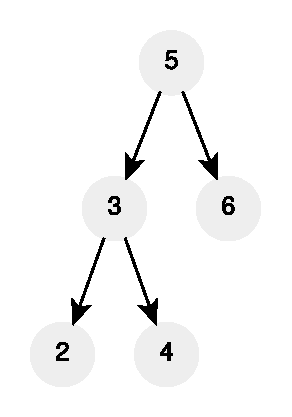
\includegraphics[width=\textwidth]{sources/remove_duplicated_sorted_array_inplace/images/example1}
%   \caption[Sample short cpation]{Sample Caption}.
%   \label{fig:remove_duplicated_sorted_array_inplace:example1} \end{figure}

\chapter{Remove duplicates in sorted array}
\label{ch:remove_duplicated_sorted_array_inplace}
\section*{Introduction}
Sorting and duplicates are the bread and butter of coding interview questions.
There are countless
problems that ask you to perform some task, or calculate an answer, where you are given either some form of sorted
input or there are duplicates involved.

In the problem described in this chapter, we are going to investigate
how we can remove duplicates from an already sorted collection of elements. This problem is easily solvable when you can use linear space but doing it \textit{in-place} and by only using constant space is slightly more challenging.




\section{Problem statement}
\begin{exercise}
\label{example:remove_duplicated_sorted_array_inplace:exercice1}
Write a function that takes a sorted array $I$ as input and returns the number of unique elements $u$ in it. 
The function should also cause all the unique elements of $I$ to appear in the first $u$ positions.



	%example1
	\begin{example}
		\label{example:remove_duplicated_sorted_array_inplace:example1}
		\hfill \\
		Given $I=\{1,1,2,2,3,3,4,5,6,6,6,6,7\}$ the function returns $7$ and $I$ is rearranged such
		that itself first $7$ elements are $\{1,2,3,4,5,6,7\}$.				
	\end{example}

	%example2
	\begin{example}
		\label{example:remove_duplicated_sorted_array_inplace:example2}
		\hfill \\
		Given $I=\{1,2,3,4\}$ the function returns $4$ and $I$ is rearranged such that its first $4$
		elements are $\{1,2,3,4\}$.	
	\end{example}
\end{exercise}

\section{Clarification Questions}

\begin{QandA}
	\begin{questionitem} \begin{question} Is the input array guaranteed to contain integers?   \end{question} 	 
    \begin{answered}
		\textit{Yes you can assume $I$ is an array of integers, but only if you are free to produce a generic solution that works for any type.}
	\end{answered} \end{questionitem}	
\end{QandA}

\section{Discussion}
\label{remove_duplicated_sorted_array_inplace:sec:discussion}
This problem behavior is remarkably similar to the function \inline{std::unique} from the STL library: it does not really remove any element from the input collection, instead, it rearranges the elements to divide the initial collection. 
The official documentation for \inline{std::unique} says that:

\quoteblock{It eliminates all except the first element from every consecutive group of equivalent elements from a range and returns a past-the-end iterator for the new logical end of the range. Removing is done by shifting the elements in the range in such a way that elements to be erased are overwritten. The relative order of the elements that remain is preserved and the physical size of the container is unchanged. Iterators pointing to an element between the new logical end and the physical end of the range are still dereferenceable, but the elements themselves have unspecified values.}

As we can see, \inline{std::unique} does not really remove or erase any element from the input collection. 
What it does instead is rearrange the elements such that the initial collection is divided into
two parts:
\begin{enumerate}
	\item the first (from the left) containing only the unique elements;
	\item the second where the duplicate elements are moved to (possibly empty).
\end{enumerate}


This function is often used in real-life applications paired with \href{https://en.cppreference.com/w/cpp/container/vector/erase2}{\inline{std::erase}} to delete the second part of the newly
arranged collection when you actually want the duplicates removed.

Listing \ref{list:remove_duplicated_sorted_array_inplace_stl} shows how we can
solve this problem with a one-liner solution using \inline{std::unique} and \inline{std::distance} from the STL. 


\lstinputlisting[language=c++, caption={One-liner solution using \inline{std::unique}.},label=list:remove_duplicated_sorted_array_inplace_stl]{sources/remove_duplicated_sorted_array_inplace/remove_duplicated_sorted_array_inplace_solution3.cpp}

The code works by first invoking \inline{std::unique} and the entire array, which causes \inline{I} to be split into two parts as described above and returns an iterator to the the first element of the second part. 
\inline{std::distance} is then used to calculate the number of elements in the first part which is the final answer.

Being able to show you can use the standard library to solve a relatively complex problem is something any interviewer is going to appreciate, however, as important as making a good first impression is, this is unlikely to be enough to clear the interview round entirely. If you use this approach
during an actual interview, the interviewer is likely to ask you to implement \inline{std::unique} and \inline{std::distance} yourself.



\subsection{Linear space solution}

As mentioned in the introduction, it is quite easy to implement this problem when you can use
linear additional space. You can think of building a list $U$ of unique elements of $I$ by:

\begin{enumerate}
	\item insert the first element of $I$;
	\item insert at the back of $U$ every element of $I$ that is not equal to the last element of $U$.
\end{enumerate}



It is important to note that $U$ does not at any moment contain duplicates. Eventually, at the end of this process, $U$ contains an ordered list of all the unique elements in $I$. All we
have to do is copy $U$ into the first $|U|$ positions of $|I|$ and return $|U|$. The complexity
of this approach is linear in time and space, as in the worst-case scenario (when $I$ does not contain duplicates) we move the entire array $I$ into $U$, and then immediately copy $U$ back into $I$. An implementation of this approach is shown below in Listing
\ref{list:remove_duplicated_sorted_array_inplace_linearspace}.

\begin{figure} 
	\centering
   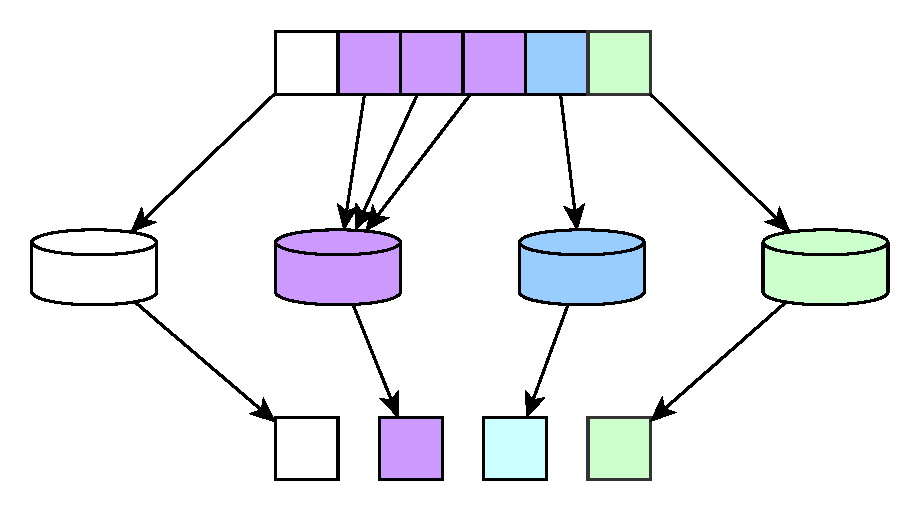
\includegraphics[width=\textwidth]{sources/remove_duplicated_sorted_array_inplace/images/intro}
   \caption[]{}
   \label{fig:remove_duplicated_sorted_array_inplace:example1} 
\end{figure}

\lstinputlisting[language=c++, caption={Linear time and space solution using \inline{std::std::unordered_set} to remember what elements have been already encountered.},label=list:remove_duplicated_sorted_array_inplace_linearspace]{sources/remove_duplicated_sorted_array_inplace/remove_duplicated_sorted_array_inplace_solution2.cpp}

\subsection{Constant Space}
\label{sec:remove_duplicated_sorted_array_inplace:constant_space}

Although we cannot do much better than spending linear time we can improve on the space used to the point where we only need a constant amount of it.
The key idea is that, because the array is sorted, equal elements will be next
to one another, therefore forming clusters of the same value. 
Eventually, $I$ has to be logically divided into
two subarrays where we only care about the content of the first part containing unique elements (no duplicates), as
there are no constraints on the content of the second part.

The algorithm proposed in this section uses a two pointer technique with which we
build the first half of $I$ one element at a time by looping through the
elements of $I$ and keeping track of two pointers:

\begin{itemize}
	\item $x$: a pointer to the last element of the first part of $I$;
	\item $y$: a pointer to the next element to be processed.
\end{itemize}

When the element pointed by $y$ is different from the element pointed by $x$, we know that we can add
$y$ to the first part of $I$. We can do that by copying $I_y$ into $I_{x+1}$ and incrementing both
$y$ and $x$ so that the next comparison would be among the last inserted element and a brand new unprocessed one.
If they are equal, however, the first part of $I$ is not going to grow and we can
safely ignore the element pointed by $y$ as we already have an instance of it (the value pointed by $X$) in the first half of $I$ already.

When all the elements of $I$ are processed ($y \geq |I|$) then the algorithm can be stopped. 
At this point
we know that $x$ is marking the end of the part of $I$ containing only unique elements. 
All we have to do is calculate and return its length. 

Listing \ref{list:remove_duplicated_sorted_array_inplace} shows an implementation of this idea.


\lstinputlisting[language=c++, caption={Linear time constant space solution.},label=list:remove_duplicated_sorted_array_inplace]{sources/remove_duplicated_sorted_array_inplace/remove_duplicated_sorted_array_inplace_solution1.cpp}

Note that with $x$ we have two important invariants:
\begin{enumerate}
	\item $x$ there are no duplicates among all the elements to the left of (including) $x$;
	\item $y$ is always larger than $x$.
\end{enumerate}

These invariants are true prior to entering the \inline{while} loop and they are true at the end of each and every iteration. It is also essential to note that the cells strictly between $x$ and $y$ can be overwritten as they must contain duplicates.

As already stated at the beginning of this section, the time complexity is linear but now, as opposed to the other solutions discussed so far, we use only constant space. 

Moreover, because we do not have to care about the state of the elements of $I$ after $x$,
we can use \href{https://en.cppreference.com/w/cpp/utility/move}{\inline{std::move}}\footnote{\inline{std::move} to indicate that an object t may be \quotes{moved from}, i.e. allowing the efficient transfer of resources from t to another object without the need for an explicit copy.} to (potentially) avoid expensive copies.

Figure \ref{fig:remove_duplicated_sorted_array_inplace:example1_process} depicts the execution of this algorithm on the input of Example \ref{example:remove_duplicated_sorted_array_inplace:example1}, where the shaded part (the left side) of the array contains all the unique elements found so far (among all the elements to the left of $y$): $x$ is a pointer to the last element of this sequence and $y$ is a pointer to the element currently processed.


\begin{figure}
	\centering
	\vspace*{0.0in}
	\begin{subfigure}[t]{0.49\textwidth}
		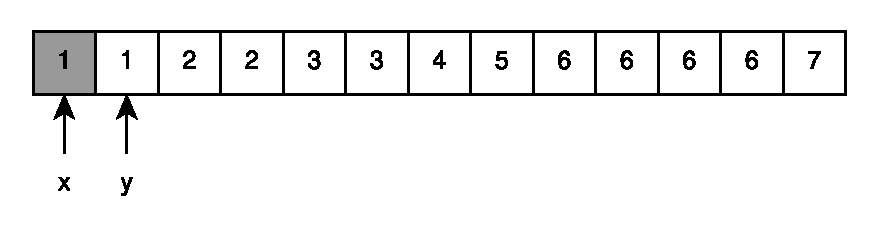
\includegraphics[width=1\linewidth]{sources/remove_duplicated_sorted_array_inplace/images/example1_1}
		\vspace*{-8mm}
		\caption{$I_x = I_y$. $y$ moved forward.}
		\label{fig:remove_duplicated_sorted_array_inplace:example1_1}
	 \end{subfigure}
	 \hfill
	 \begin{subfigure}[t]{0.49\textwidth}
		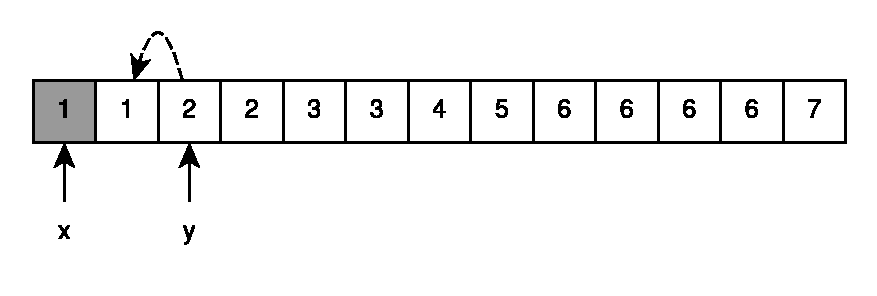
\includegraphics[width=1\linewidth]{sources/remove_duplicated_sorted_array_inplace/images/example1_2}
		\vspace*{-8mm}
		\caption{$1 = I_x \neq I_y = 2$. $I_y$ copied into $I_{x+1}$. $y$ and $x$ are moved forward.}
		\label{fig:remove_duplicated_sorted_array_inplace:example1_2}
	 \end{subfigure}
	 \hfill
	 \begin{subfigure}[t]{0.49\textwidth}
		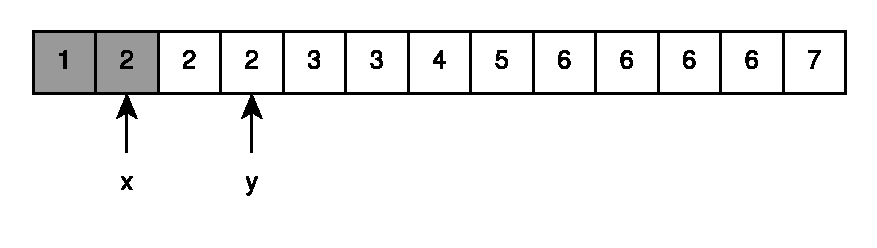
\includegraphics[width=1\linewidth]{sources/remove_duplicated_sorted_array_inplace/images/example1_3}
		\vspace*{-8mm}
		\caption{$I_x = I_y$. $y$ only moved forward.}
		\label{fig:remove_duplicated_sorted_array_inplace:example1_3}
	 \end{subfigure}
	 \hfill
	 \begin{subfigure}[t]{0.49\textwidth}
		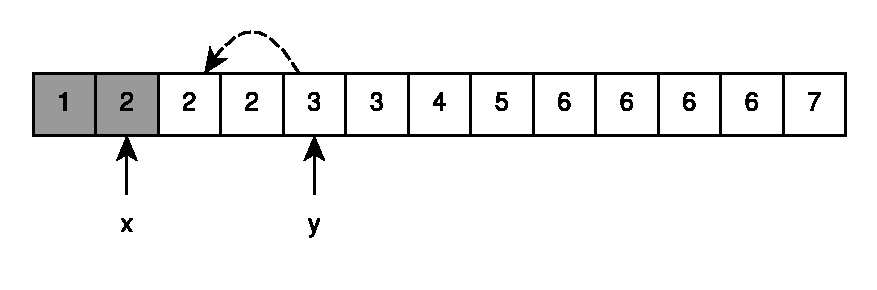
\includegraphics[width=1\linewidth]{sources/remove_duplicated_sorted_array_inplace/images/example1_4}
		\vspace*{-8mm}
		\caption{$2 = I_x \neq I_y = 3$. $I_y$ copied into $I_{x+1}$. $y$ and $x$ are moved forward.}
		\label{fig:remove_duplicated_sorted_array_inplace:example1_4}
	 \end{subfigure}
	 \hfill
	 \begin{subfigure}[t]{0.49\textwidth}
		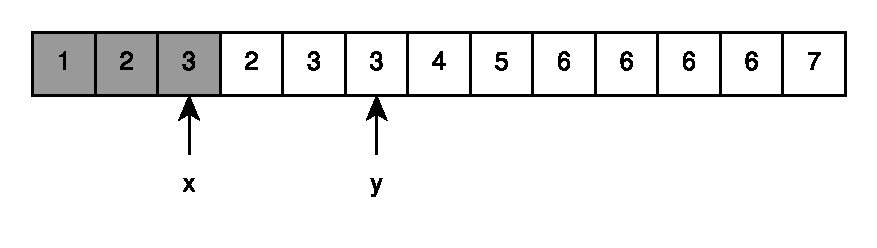
\includegraphics[width=1\linewidth]{sources/remove_duplicated_sorted_array_inplace/images/example1_5}
		\vspace*{-8mm}
		\caption{$I_x = I_y$. $y$ moved forward.}
		\label{fig:remove_duplicated_sorted_array_inplace:example1_5}
	 \end{subfigure}
	 \hfill
	 \begin{subfigure}[t]{0.49\textwidth}
		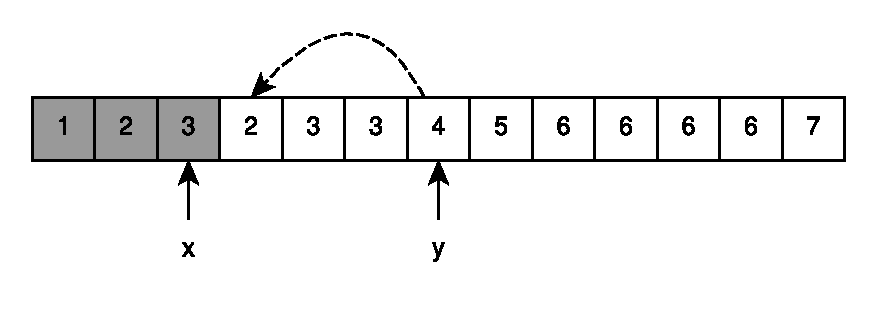
\includegraphics[width=1\linewidth]{sources/remove_duplicated_sorted_array_inplace/images/example1_7}
		\vspace*{-8mm}
		\caption{$3 = I_x \neq I_y = 4$. $I_y$ copied into $I_{x+1}$. $y$ and $x$ are moved forward.}
		\label{fig:remove_duplicated_sorted_array_inplace:example1_6}
	 \end{subfigure}
	 \hfill
	 \begin{subfigure}[t]{0.49\textwidth}
		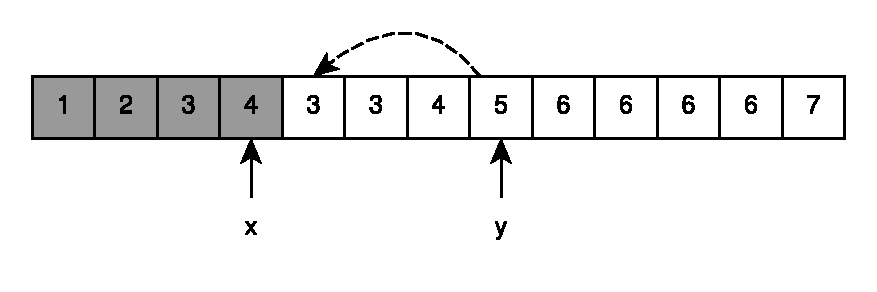
\includegraphics[width=1\linewidth]{sources/remove_duplicated_sorted_array_inplace/images/example1_8}
		\vspace*{-8mm}
		\caption{$4 = I_x \neq I_y = 5$. $I_y$ copied into $I_{x+1}$. $y$ and $x$ are moved forward.}
		\label{fig:remove_duplicated_sorted_array_inplace:example1_6}
	 \end{subfigure}
	 \hfill
	 \begin{subfigure}[t]{0.49\textwidth}
		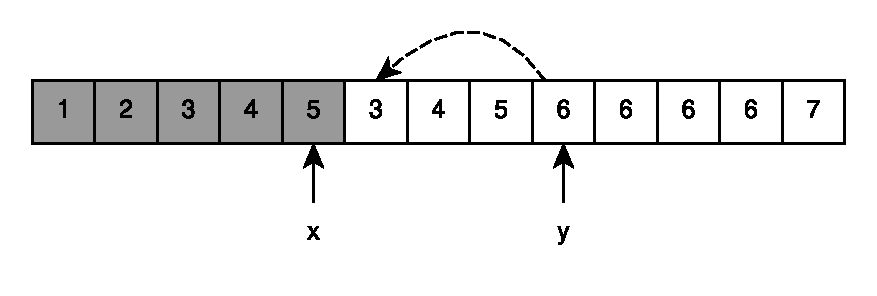
\includegraphics[width=1\linewidth]{sources/remove_duplicated_sorted_array_inplace/images/example1_10}
		\vspace*{-8mm}
		\caption{$5 = I_x \neq I_y = 6$. $I_y$ copied into $I_{x+1}$. $y$ and $x$ are moved forward.}
		\label{fig:remove_duplicated_sorted_array_inplace:example1_6}
	 \end{subfigure}
	 \hfill
	 \begin{subfigure}[t]{0.49\textwidth}
		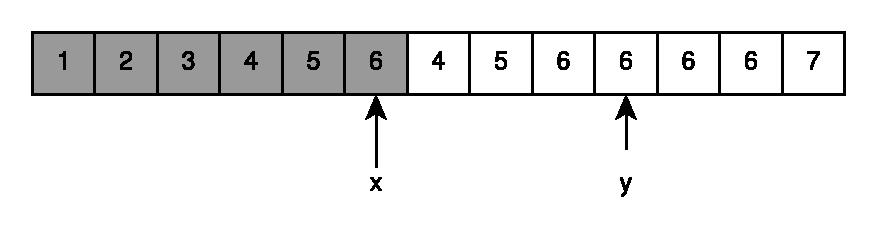
\includegraphics[width=1\linewidth]{sources/remove_duplicated_sorted_array_inplace/images/example1_11}
		\vspace*{-8mm}
		\caption{$I_x = I_y$. $y$ moved forward.}
		\label{fig:remove_duplicated_sorted_array_inplace:example1_6}
	 \end{subfigure}
	 \hfill
	 \begin{subfigure}[t]{0.49\textwidth}
		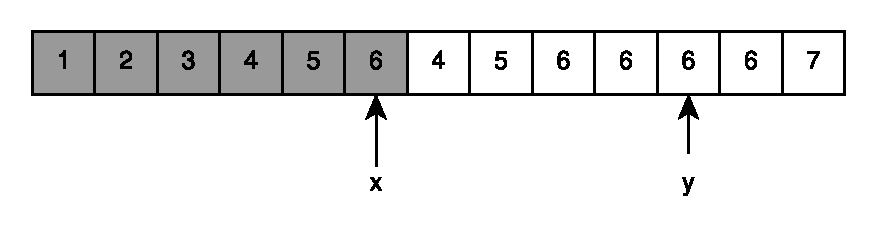
\includegraphics[width=1\linewidth]{sources/remove_duplicated_sorted_array_inplace/images/example1_12}
		\caption{$I_x = I_y$. $y$ moved forward.}
		\label{fig:remove_duplicated_sorted_array_inplace:example1_6}
	 \end{subfigure}
	 \hfill
	 \begin{subfigure}[t]{0.49\textwidth}
		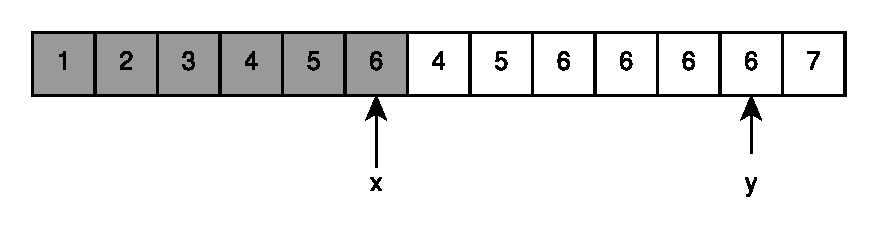
\includegraphics[width=1\linewidth]{sources/remove_duplicated_sorted_array_inplace/images/example1_13}
		\vspace*{-8mm}
		\caption{$I_x = I_y$. $y$ moved forward.}
		\label{fig:remove_duplicated_sorted_array_inplace:example1_6}
	 \end{subfigure}
	 \hfill
	 \begin{subfigure}[t]{0.49\textwidth}
		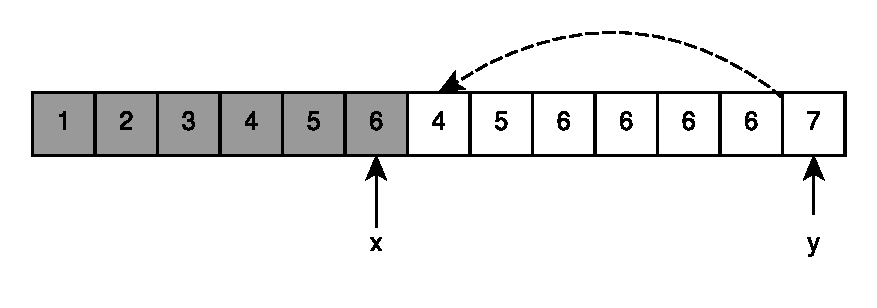
\includegraphics[width=1\linewidth]{sources/remove_duplicated_sorted_array_inplace/images/example1_14}
		\vspace*{-8mm}
		\caption{$6 = I_x \neq I_y = 7$. $I_y$ copied into $I_{x+1}$. $y$ and $x$ are moved forward.}
		\label{fig:remove_duplicated_sorted_array_inplace:example1_6}
	 \end{subfigure}
	 \hfill
	 \begin{subfigure}[t]{0.49\textwidth}
		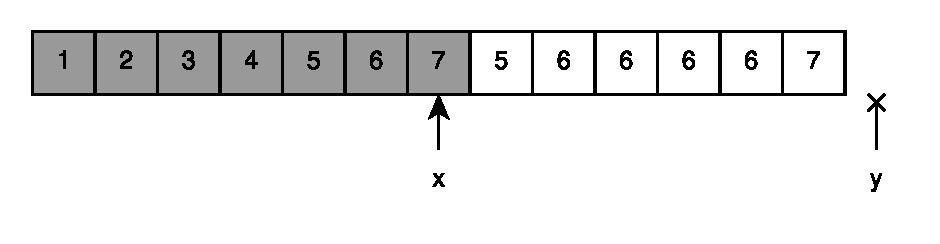
\includegraphics[width=1\linewidth]{sources/remove_duplicated_sorted_array_inplace/images/example1_15}
		\vspace*{-8mm}
		\caption{$y$ is outside the range of valid elements of $I$. The algorithm stops.}
		\label{fig:remove_duplicated_sorted_array_inplace:example1_6}
	 \end{subfigure}
\caption{Execution of the algorithm implemented in Listing
 \ref{list:remove_duplicated_sorted_array_inplace} on the input of the Example
 \ref{example:remove_duplicated_sorted_array_inplace:example1}. The shaded part of the array
 contains all the unique elements processed so far. $x$ is a pointer to the last element of this
 sequence. $y$ is a pointer to the element currently processed.}
\label{fig:remove_duplicated_sorted_array_inplace:example1_process}
\end{figure}

\section{Common Variations}
\subsection{Max $2$ duplicates allowed}
In this section, we will have a look at a common variation of the main problem of this lesson, which differs from it on the basis that each element can now appear at \textbf{most twice} in the final rearrangement of $I$.

\begin{exercise}
Write a function that  -  given a sorted array $I$  - removes all the 
duplicates in such a way that an element appears \textbf{at most twice} and with all the valid elements being located at the beginning of $I$ itself.
The function returns the number of valid elements in $I$.
	
	\label{example:remove_duplicated_sorted_array_inplace:exercice2}
	
		%example1
		\begin{example}
			\label{example:remove_duplicated_sorted_array_inplace_variation1:example1}
			\hfill \\
			Given $I=\{1,1,2,2,3,3,4,5,6,6,6,6,7\}$ the function returns $11$ and $I$ is rearranged such
			that itself first $11$ elements are $\{1,1,2,2,3,3,4,5,6,6,7\}$.				
		\end{example}
	
		%example2
		\begin{example}
			\label{example:remove_duplicated_sorted_array_inplace_variation1:example2}
			\hfill \\
			Given $I=\{1,2,3,4\}$ the function returns $4$ and $I$ is rearranged such that its first $4$
			elements are $\{1,2,3,4\}$.	
		\end{example}
\end{exercise}

\subsection{Discussion}

This variant can be solved with minimal changes to the solution presented for the main problem.
We can modify the code shown in the Section \ref{sec:remove_duplicated_sorted_array_inplace:constant_space} so that we keep track of the number of repetitions we have already inserted for a given element.
This can be implemented as shown in Listing \ref{list:remove_duplicated_sorted_array_inplace_max_two}.

\lstinputlisting[language=c++, caption={Linear time constant space solution to the variation where at most two duplicates are allowed.},label=list:remove_duplicated_sorted_array_inplace_max_two]{sources/remove_duplicated_sorted_array_inplace/remove_duplicated_sorted_array_inplace_solution4.cpp}


Note that the meaning of the variables $x$ and $y$ did not change, and that here we use the variable \inline{consecutive} to keep track of the number of times the element pointed by \inline{x} appears in the array \inline{A}. 
If the element pointed by \inline{y} is equal to the element pointed by \inline{x} (we have a duplicate), then we decide whether to insert it or not based on the value of the variable \inline{consecutive}:
\begin{itemize}
	\item If it appears already more than $1$ times we discard it;
	\item otherwise, we copy it to the cell at index $x+1$ and increment \inline{consecutive}.
\end{itemize}

The time and space complexity of this approach is $O(|I|)$ and $O(1)$, respectively.

\subsection{Max $k$ duplicates allowed}
This variation is also a quite common and is basically a generalization of the problems above where now each element can appear $k$ times.
Note that when $k= 1$ and $k=2$ this problem is equivalent to the Problems \ref{example:remove_duplicated_sorted_array_inplace:exercice1} and \ref{example:remove_duplicated_sorted_array_inplace:exercice2}.
The solution for this variation is not discussed here as it can be easily derived from the solution to the Problem \ref{example:remove_duplicated_sorted_array_inplace:exercice1}.

\begin{exercise}
Write a function that  - given a sorted array $I$  - removes all the 
duplicates in such a way an element appears at most twice and with all the valid elements being located at the beginning of the $I$ itself.
The function returns the number of valid elements in $I$.
	
	\label{example:remove_duplicated_sorted_array_inplace_variation:exercice3}
	
		%example1
		\begin{example}
			\label{example:remove_duplicated_sorted_array_inplace_variation2:example1}
			\hfill \\
			Given $I=\{1,1,2,2,3,3,4,5,6,6,6,6,7\}$ and $k=3$ the function returns $12$ and $I$ is rearranged such
			that itself first $1$ elements are $\{1,1,2,2,3,3,4,5,6,6,6,7\}$. Notice the extra $6$ w.r.t. the Example \ref{example:remove_duplicated_sorted_array_inplace_variation1:example1}.
		\end{example}
	
		%example2
		\begin{example}
			\label{example:remove_duplicated_sorted_array_inplace_variation2:example2}
			\hfill \\
			Given $I=\{1,1,1,1,1,1,1,2,2,3,3,3,4,4\}$ and $k=5$ the function returns $13$ and $I$ is rearranged such that its first $13$
			elements are $\{1,1,1,1,1,2,2,3,3,3,3,4,4\}$.	
		\end{example}
	\end{exercise}